
% This text is proprietary.
% It's a part of presentation made by myself.
% It may not used commercial.
% The noncommercial use such as private and study is free
% Sep. 2005 
% Author: Sascha Frank 
% University Freiburg 
% www.informatik.uni-freiburg.de/~frank/


\documentclass{beamer}

\usepackage{color}
\newcommand{\avg}[1]{\overline{#1}}
\newcommand{\fluct}[1]{#1'}
\newcommand{\red}[1]{\textcolor{red}{#1}}

\usepackage{graphicx}
\usepackage{natbib}
\usepackage{tikz}

\pgfdeclareimage[width=0.6\paperwidth]{mybackground}{TEX/FIGS/channel.png}

\setbeamertemplate{title page}{

  \begin{picture}(0,0)


    \put(40,-150){%
      \pgfuseimage{mybackground}
    }

    \put(10,-40){%
      \begin{minipage}[b][45mm][t]{226mm}
        \usebeamerfont{title}{\huge\textbf\inserttitle\par}
        \hspace{3cm} - An introduction \\
      \end{minipage}
    }

  \end{picture}

}

\begin{document}
\title{Simulation of Turbulent Flows}   
\author{Gregor Olenik} 
\date{\today} 

\frame{\titlepage} 

\frame{\frametitle{Motivation} 
      \begin{columns}
    \column{0.5\textwidth}
    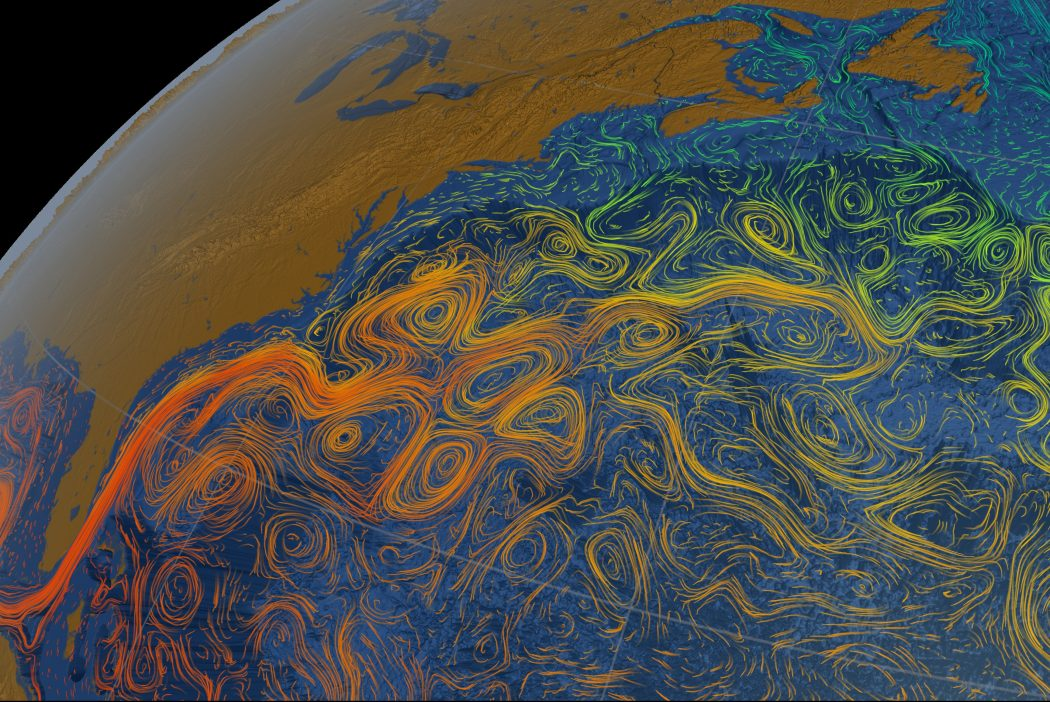
\includegraphics[width=\textwidth]{TEX/FIGS/ocean.jpg}
    Casey \cite{Casey}

    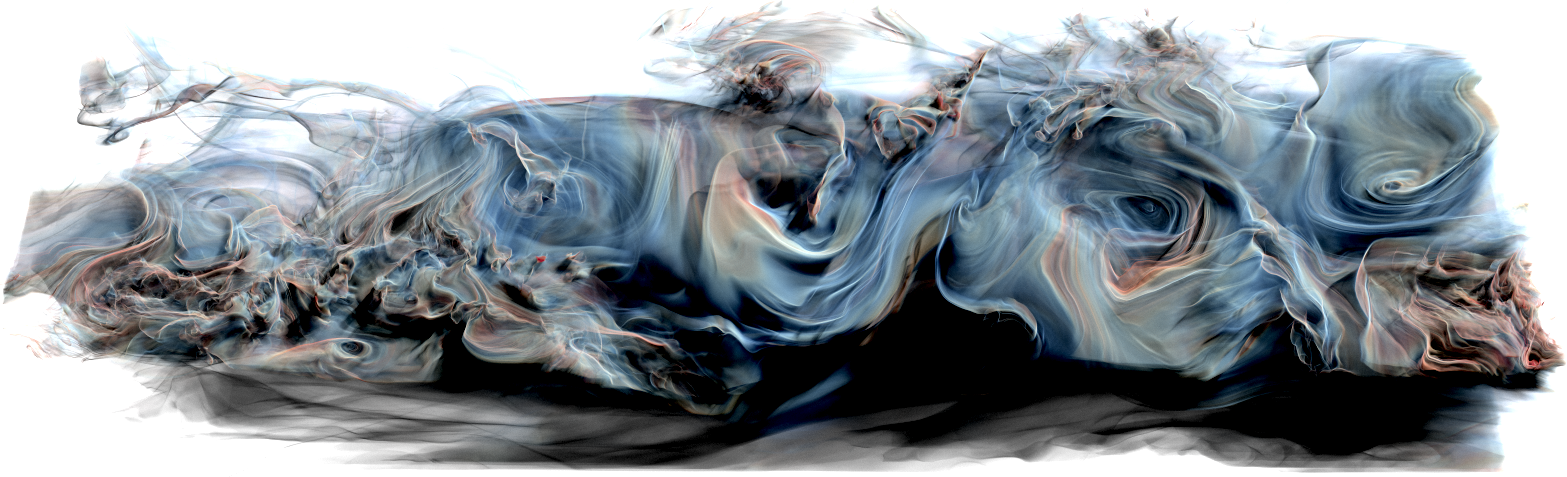
\includegraphics[width=\textwidth]{TEX/FIGS/atmosphere_c.png}
    G\"unther et al. \cite{Guenther}
    \column{0.5\textwidth}

        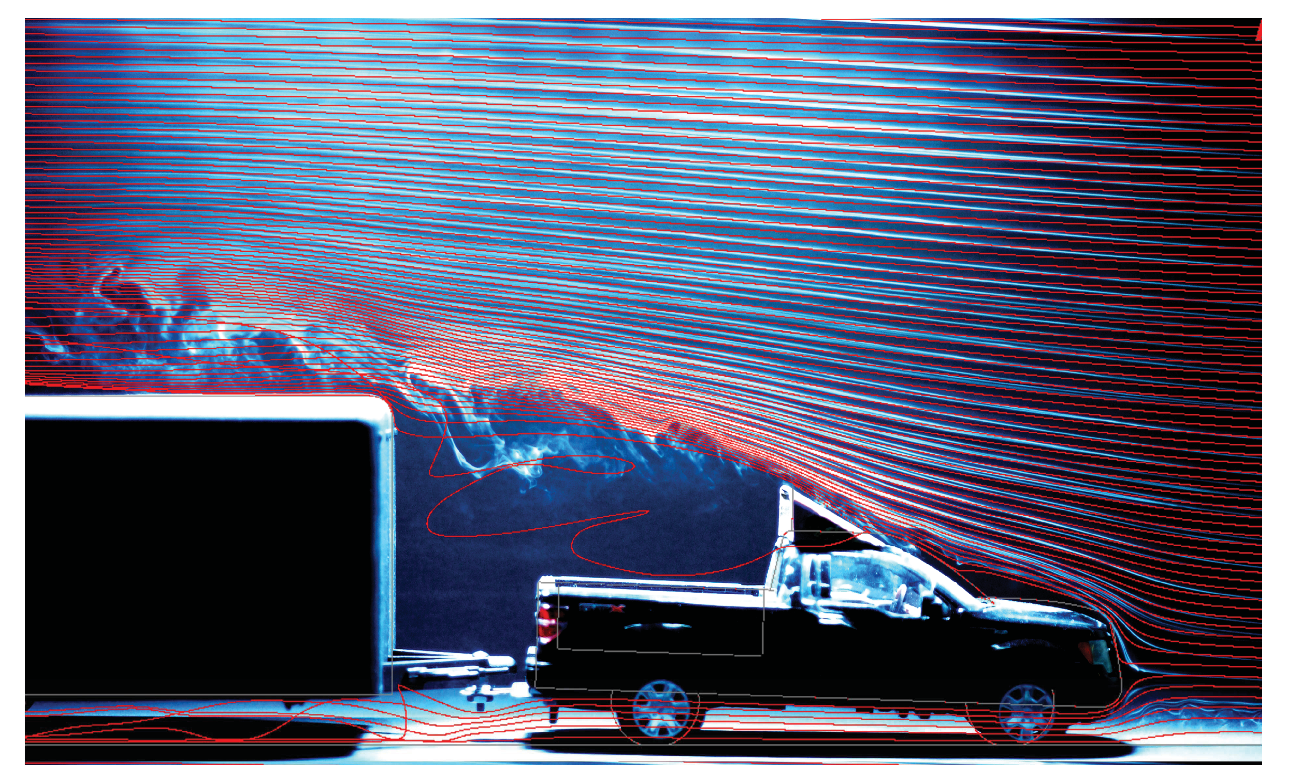
\includegraphics[width=\textwidth]{TEX/FIGS/car_c.png}
      Boyer et al. \cite{Boyer}
      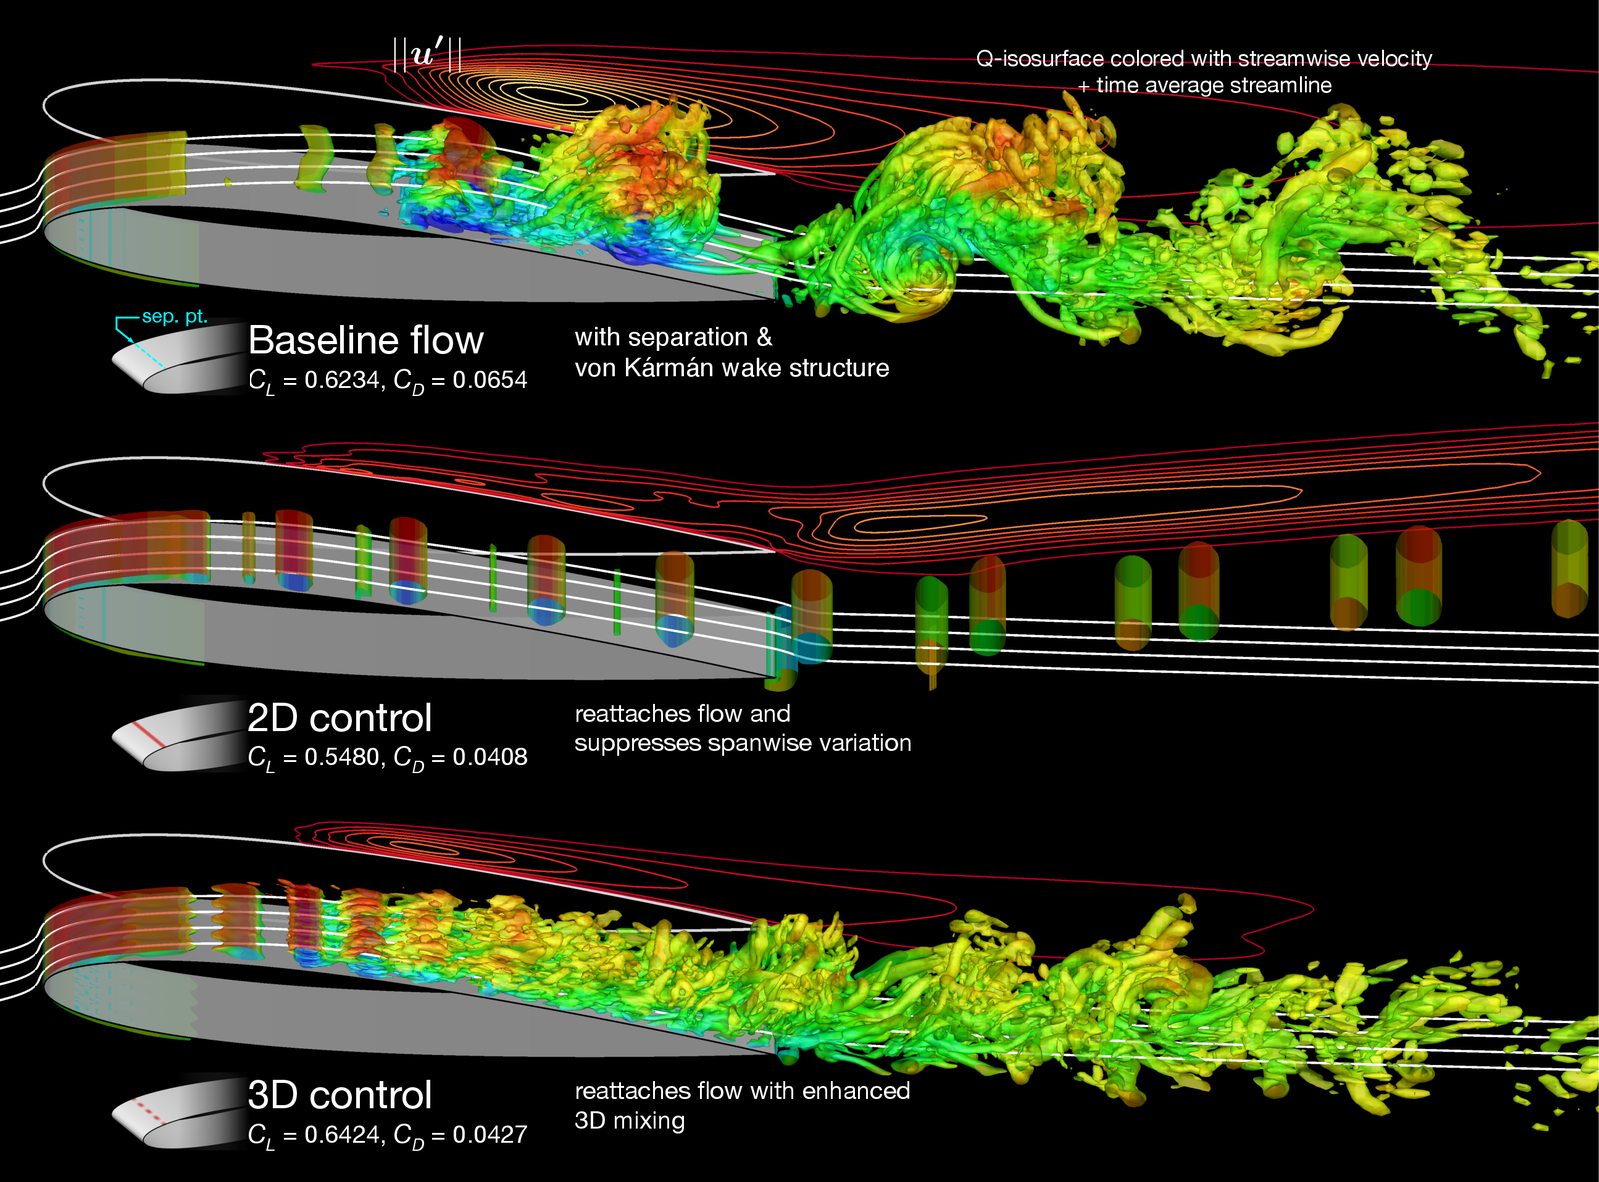
\includegraphics[width=\textwidth]{TEX/FIGS/wing_c.png}
      Yeh et al. \cite{yeh}
      \end{columns}
}

\frame{\frametitle{Content} 

\begin{itemize}
\item[-] Fundamentals of Simulation
\item[-] What is turbulence  
\item[-] Consequences of Turbulence
\item[-] Basic Modelling Approaches
\item[-] Summary and Outlook
\end{itemize} 
}

\frame{\frametitle{Fundamentals Simulation}

  \begin{columns}

    \column{0.6\textwidth}
    \small
  \begin{equation}
  \frac{\partial u_i}{\partial t} + u_j \frac{\partial u_i}{\partial x_j}
  = f_i 
  - \frac{1}{\rho} \frac{\partial p}{\partial x_i}
  + \nu \frac{\partial^2 u_i}{\partial x_j \partial x_j}
  \end{equation}

  \column{0.4\textwidth}
  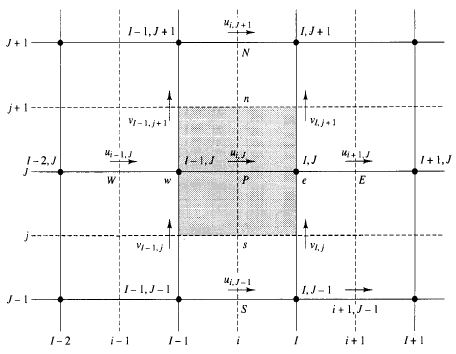
\includegraphics[width=\textwidth]{TEX/FIGS/grid.jpg}
  \end{columns}
\begin{itemize}
\item[-] Integration over cell surfaces of computational grid
\item[-] Application of Gauss theorem
\item[-] Interpolation of face values
\item[-] Setup of boundary conditions
\item[-] Linearisation
\item[-] Assembly of matrix coefficients
\end{itemize} 
}

\frame{\frametitle{What is turbulence}
  \begin{columns}
    \column{0.5\textwidth}
    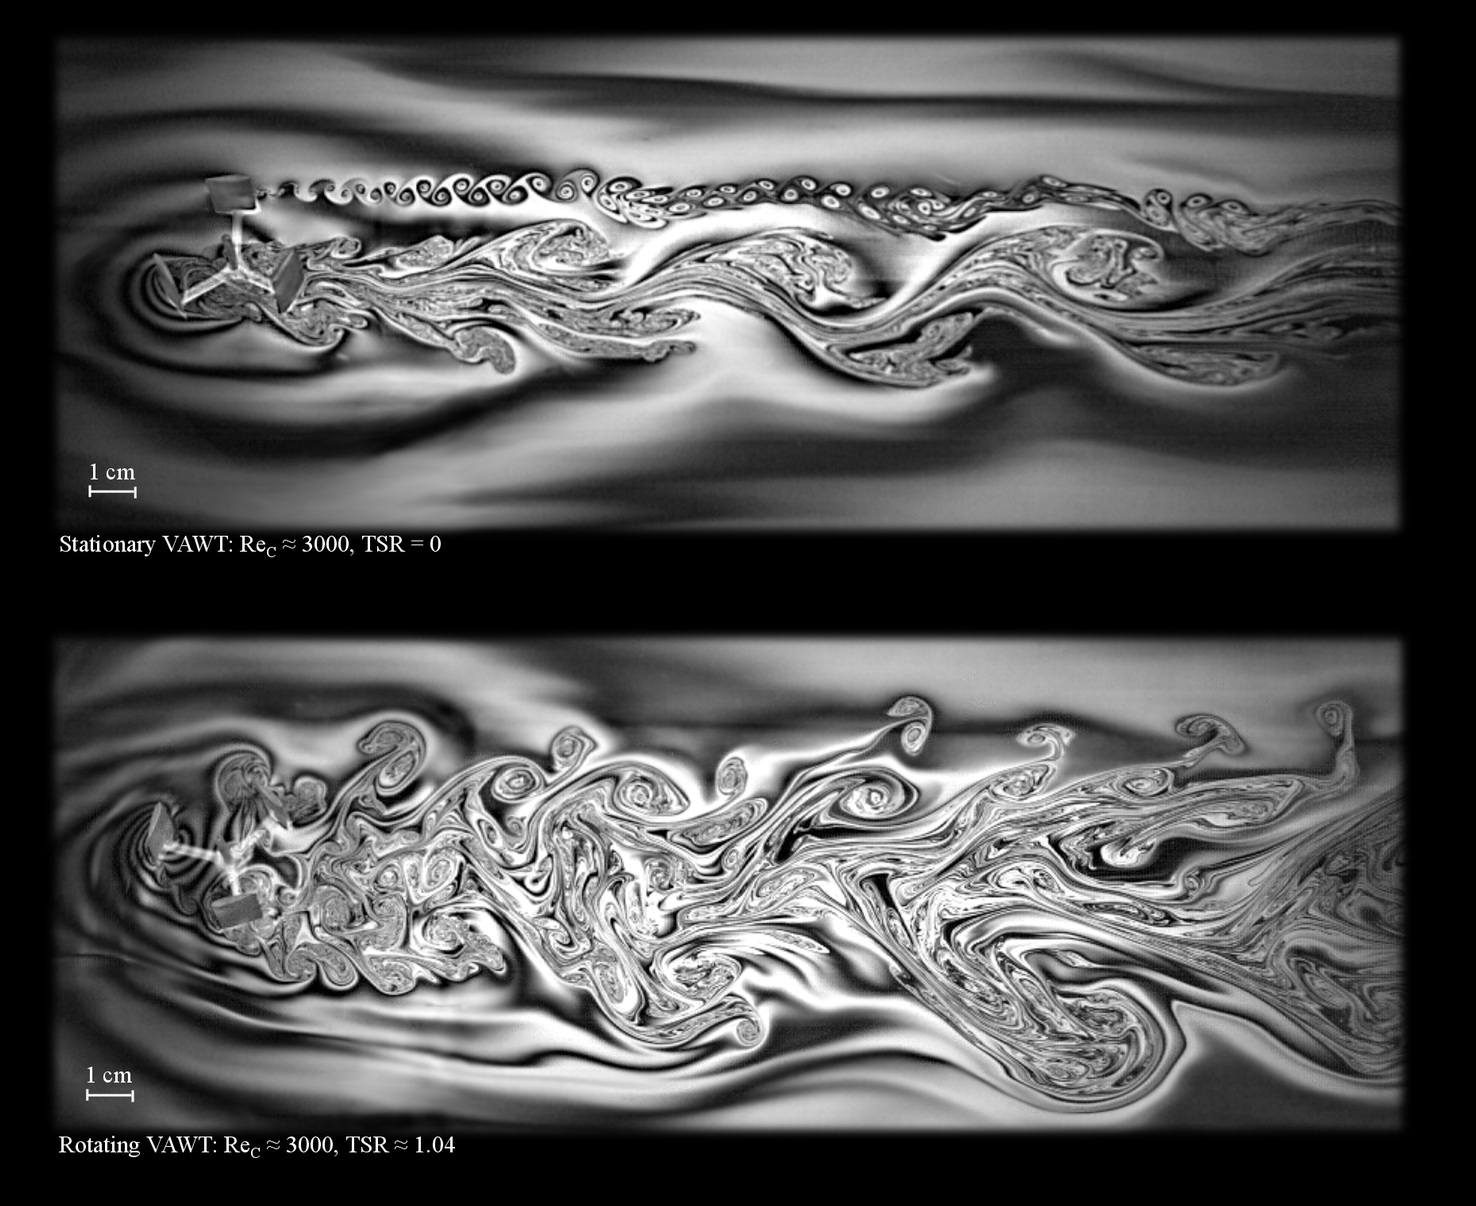
\includegraphics[width=\textwidth]{TEX/FIGS/transition_c.png}
    Araya and Dabiri \cite{Araya}
    \column{0.5\textwidth}
    Tennekes and Lumley \cite{tennekes}
\begin{itemize}
\item[-] Irregularity
\item[-] Diffusivity
\item[-] Dissipative
\item[-] Large Reynolds numbers, $\text{Re}=uL/\nu=$ momentum/viscous forces
\item[-] 3D and transient
\end{itemize}
\end{columns}
}

\frame{\frametitle{The Role of Vortices}
  \begin{columns}
  %% A posteriori analysis of low-pass spatial filters for approximate deconvolution large eddy simulations of homogeneous incompressible flows
    \column{0.66\textwidth}
  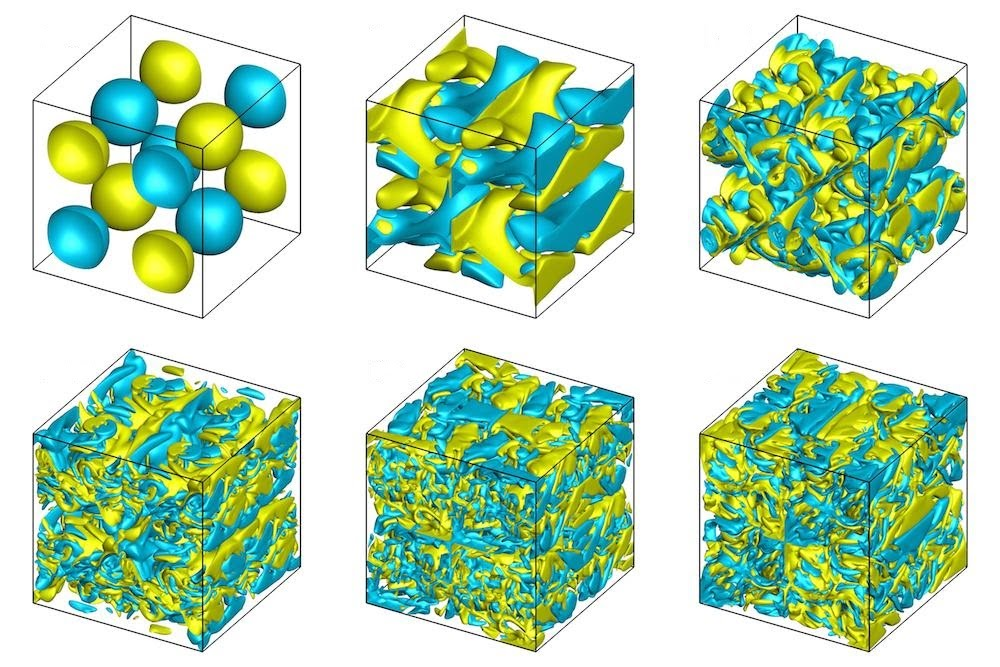
\includegraphics[width=\textwidth]{TEX/FIGS/tgv.jpg}
  San et al. \cite{san}
  \begin{itemize}
  \item[-]  $\eta/L=\text{Re}^{-3/4}$
  \item[-]  $n_{\text{Cells}} = f(\text{Re}^{9/4})$, $n_{\text{TS}} = f(\text{Re}^{9/4})$
  \end{itemize}
  %% Complete measurement of helicity and its dynamics in vortex tubes
  \column{0.34\textwidth}
  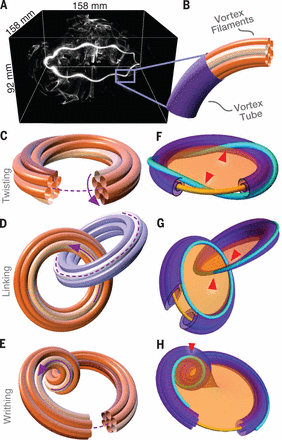
\includegraphics[width=\textwidth]{TEX/FIGS/vortex.png}
  Scheeler et al. \cite{scheeler}
  \end{columns}
}


\frame{\frametitle{Consequences of Turbulence }

  \begin{columns}
    \column{0.5\textwidth}
    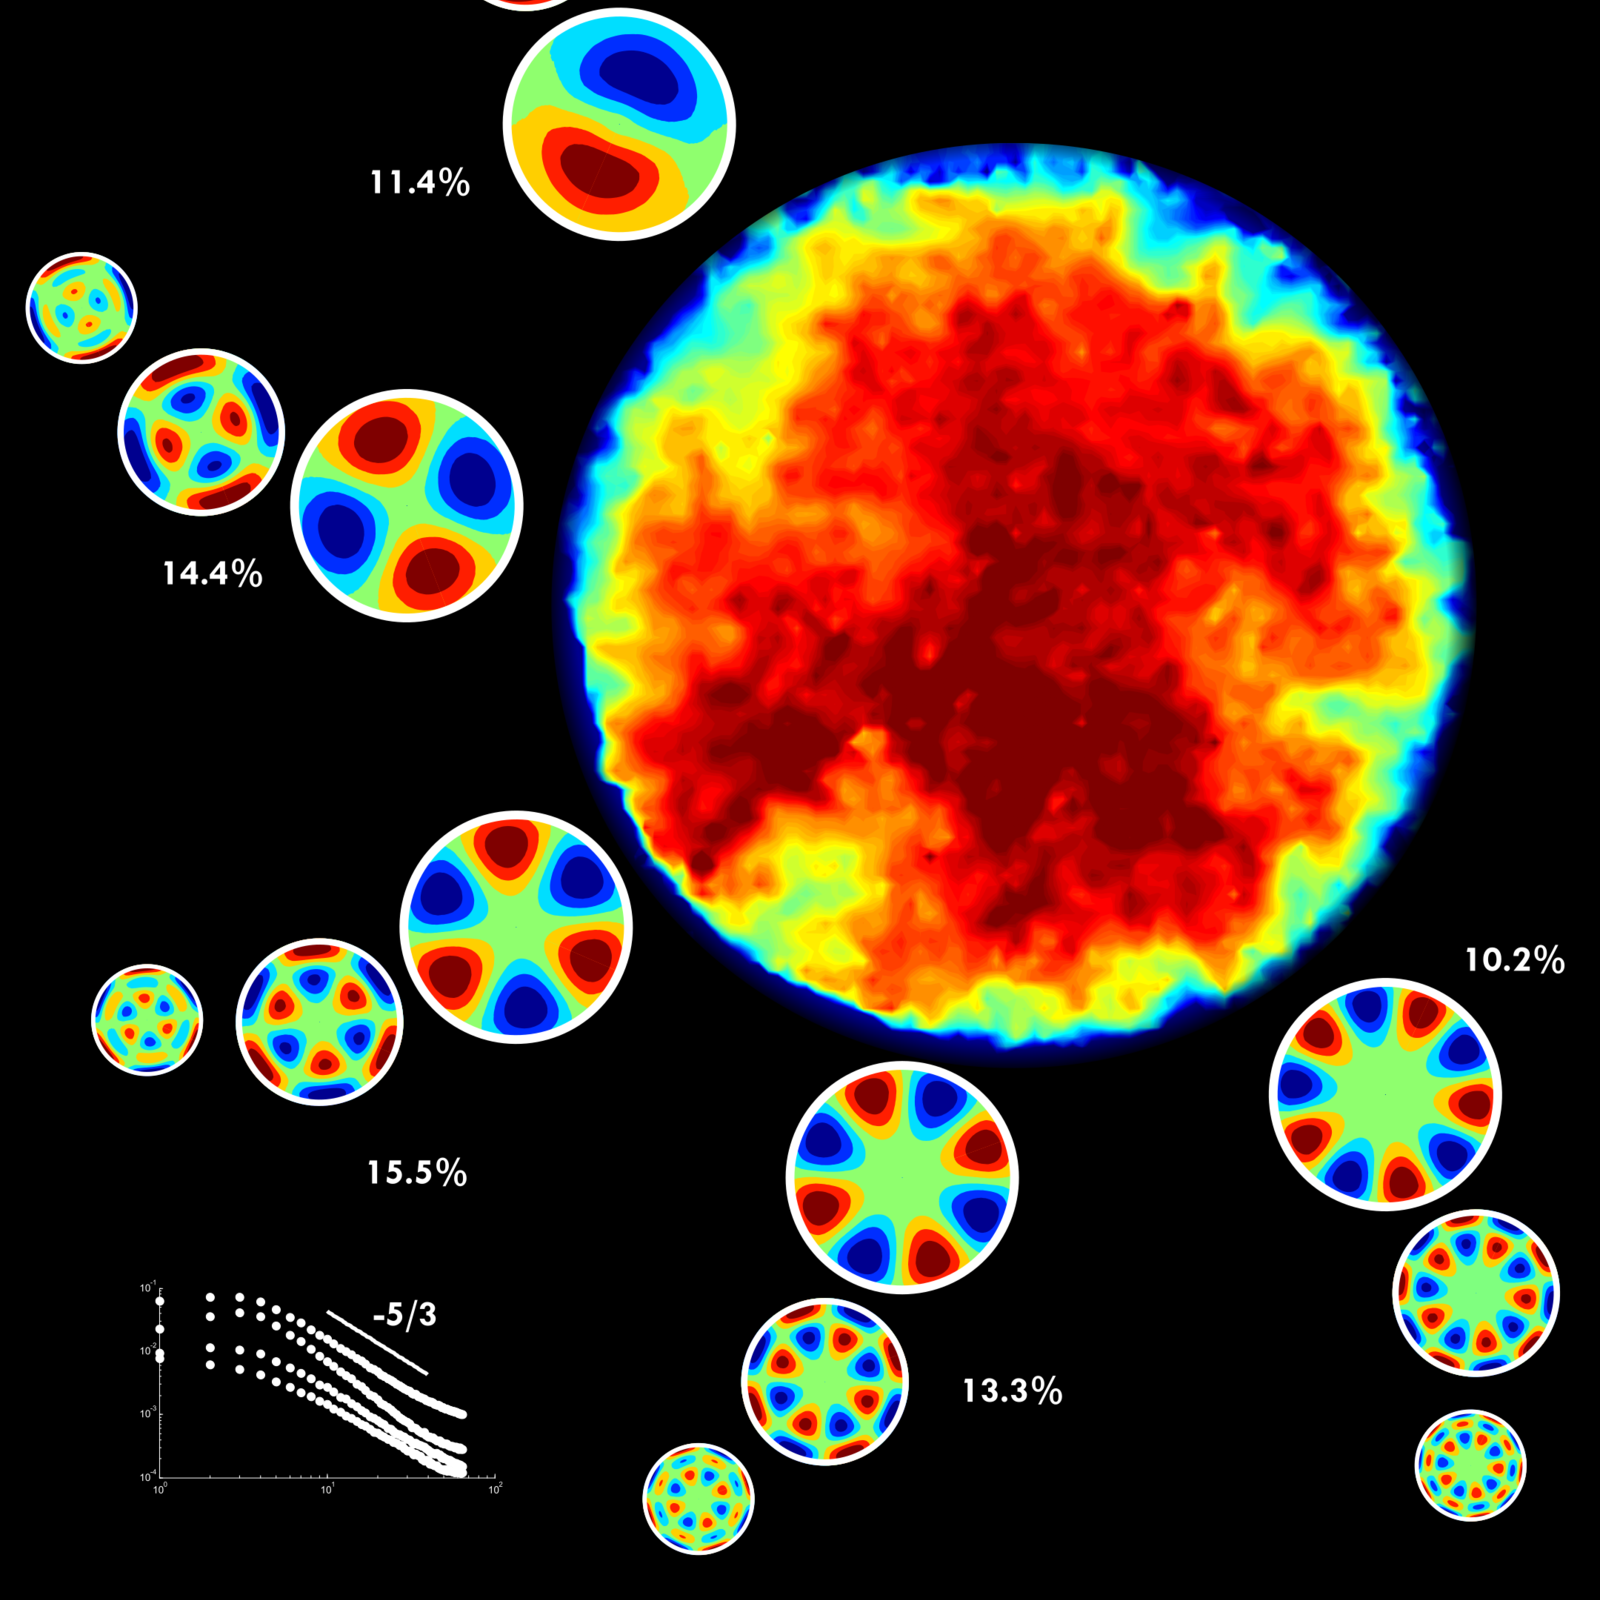
\includegraphics[width=\textwidth]{TEX/FIGS/pipe_c.png}
    Floryan et al. \cite{Floryan}
    \column{0.5\textwidth}
DNS of Ahn et al. \cite{ahn}
\begin{tabular}{|c|c|}
\hline
$n_{\text{cores}}$ & $4906$  \\ \hline
$n_{\text{cells}}$ & $30x10^9$ \\ \hline
$s_{\text{TS}}$   & $1TB$ \\
\hline
\end{tabular}

\begin{itemize}
\item[-]  Air viscosity of air $1.0x10^{-5}$
\item[-]  Diameter of $0.1$m
\end{itemize}

\begin{tabular}{|c|c|}
  \hline
  $u_{\text{b}}$ & $20$ m/s  \\ \hline
  $L$ & $1$m \\ \hline
  $n_{\text{TS}}$   & $150$k \\
  \hline
\end{tabular}

\end{columns}
}


\frame{\frametitle{Basic Turbulence Modelling Approaches - RANS}

  \begin{itemize}
  \item[-] Complete $\avg{\avg{\phi}} = \avg{\phi}$
  \item[-] Uncorrelated $\avg{\phi\psi} \neq \avg{\phi}~\avg{\psi}$
  \item[-] Distributive $\avg{\phi+\psi}=\avg{\psi}+\avg{\phi}$
  \item[-] Reynolds decomposition  $\phi(t)=\avg{\phi} + \fluct{\phi}(t)$ $\avg{\fluct{\phi}} = 0$,
  \end{itemize}

  \begin{equation}
   \rho \frac{\partial \bar{u_i}}{\partial t} 
    + \rho\bar{u}_j  \frac{\partial \bar{u}_i }{\partial x_j}
    = \rho \bar{f}_i
    + \frac{\partial}{\partial x_j} 
    \left[ - \bar{p}\delta_{ij} 
      + \mu \left( \frac{\partial \bar{u}_i}{\partial x_j} + \frac{\partial \bar{u}_j}{\partial x_i} \right)
      \red{- \rho \overline{u_i^\prime u_j^\prime}} \right ].
  \end{equation}
  \begin{equation}
-\overline{u_i^\prime u_j^\prime} = \nu_t\left (\frac{\partial\overline{u_i}}{\partial x_j}+\frac{\partial\overline{u_j}}{\partial x_i} \right )-\frac{2}{3}k \delta_{ij}
  \end{equation}
  \begin{equation}
    \rho \frac{\partial \bar{u_i}}{\partial t} 
    + \rho\bar{u}_j  \frac{\partial \bar{u}_i }{\partial x_j}
    = \rho \bar{f}_i
    + \frac{\partial}{\partial x_j} 
    \left[ - \bar{p^*}\delta_{ij} 
      + \left ( \mu + \mu_t \right ) \left( \frac{\partial \bar{u}_i}{\partial x_j} + \frac{\partial \bar{u}_j}{\partial x_i} \right)
      \right ].
  \end{equation}
}

\frame{\frametitle{Basic Turbulence Modelling Approaches - k-$\epsilon$ Modell}
\begin{equation}
\mu_t = \rho C_{\mu} \frac{k^2}{\epsilon}
\end{equation}


\begin{equation}
\frac{\partial}{\partial t} (\rho k) + \frac{\partial}{\partial x_i} (\rho k u_i) = \frac{\partial}{\partial x_j} \left[ \left(\mu + \frac{\mu_t}{\sigma_k} \right) \frac{\partial k}{\partial x_j}\right] + P_k + P_b - \rho \epsilon - Y_M + S_k
\end{equation}

\begin{equation}
\frac{\partial}{\partial t} (\rho \epsilon) + \frac{\partial}{\partial x_i} (\rho \epsilon u_i) = \frac{\partial}{\partial x_j} \left[\left(\mu + \frac{\mu_t}{\sigma_{\epsilon}} \right) \frac{\partial \epsilon}{\partial x_j} \right] + C_{1 \epsilon}\frac{\epsilon}{k} \left( P_k + C_{3 \epsilon} P_b \right) - C_{2 \epsilon} \rho \frac{\epsilon^2}{k} + S_{\epsilon}
\end{equation}
}

\frame{\frametitle{Summary}

  \begin{itemize}
  \item[-] Replaced a system of 3 instantaneous transport equations by a 5 steady;
    state transport equations
  \item[-] Since fluctuations are modelled a coarse mesh suffices;
  \item[-] For time averaged RANS only a fraction of iterations are needed;
  \end{itemize}

  \begin{columns}
  \column{0.5\textwidth}
  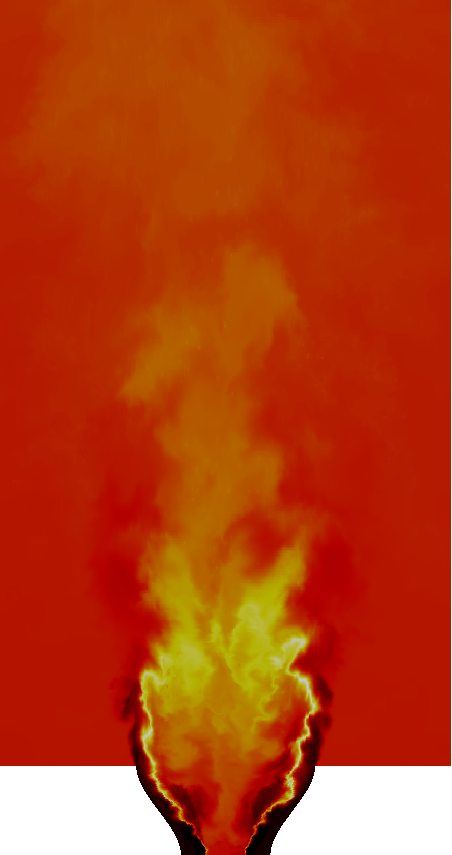
\includegraphics[width=0.5\textwidth]{TEX/FIGS/IFRFTquarl.png} \\
  Olenik et al. \cite{Olenik2015}
  \column{0.5\textwidth}
  \includegraphics[width=0.65\textwidth]{TEX/FIGS/CRIEPISnapshotCold.png} \\
  Stein et al. \cite{stein_2012}
  \end{columns}
}
\frame{\frametitle{Outlook}
  \begin{itemize}
  \item[-] Ginkgo as solver for OpenFOAM
  \end{itemize}
  }

\bibliographystyle{alpha}
\bibliography{main} 

\end{document}

